\chapter{Vertailu\label{vertailu}}

Kaksi- ja monivaiheisia kirjautumistapoja on todettu olevan monia erilaisia menetelmiä. Myös käyttötarkoituksia, joissa näitä menetelmiä käytetään, on olemassa monia. Seuraavaksi vertaillaan kuutta varmentamismenetelmää neljässä eri käyttötarkoituksessa. Vertailuun ei ole valittu yksittäisiä käyttötarkoituksia kuten yksittäistä verkkosivua vaan yleisimpiä kategorioita, jotka kuvaavat laajempaa käyttötarkoitus joukkoa. Valitut kirjautumismenetelmät sekä käyttötarkoitukset pyrkivät kuvaamaan monipuolisesti varmentamismenetelmien soveltuvuutta eri käyttötarkoituksissa. 

Vertailuun valitut varmentamismenetelmät ovat SMS varmenne, Kertakäyttöiset koodit, Fyysinen avain, Mobiilisovellus, Sähköposti ja Verkkopankkitunnukset.

Pankit vaativat nykyään verkkopankkitunnuksen lisäksi kaksivaiheisen tunnistautumisen. Kaksivaiheisia tunnistautumistapoja, joita pankit tarjoavat ovat mobiilisovellus, kertakäyttöiset koodit, tekstiviesti vahvistus sekä myös muita menetelmiä \citep{nordea_tunnistautuminen} \citep{op_tunnistautuminen} \citep{spankki_tunnistautuminen}. Verkkopankkiin kirjautumisessa yhdistyy kaksi vertailtavaa varmentamismenetelmää. Tämä ei ole suotuisaa, joten oletuksena on, että verkkopankkitunnus koostuu pankkitunnuksesta sekä kirjautumiseen vaadittavasta kaksivaiheisesta tunnistautumisesta. Muut vertailtavat varmentamismenetelmät koostuvat käyttäjätunnuksesta sekä varmentamismenetelmästä. 


Vertailun ensimmäinen vertailtava käyttötarkoitus on verkkosivut. Verkkosivuilla tarkoitetaan yleisellä tasolla verkossa olevia sivustoja tai palveluita kuten sähköposti ja sosiaaliset mediat, joihin käyttämiseen vaaditaan kirjautumista

Toinen vertailtava käyttötarkoitus on pankkipalvelut. Verkkopankkien käyttäminen laskujen maksamiseen on yleistynyt merkittävästi tämän vuosituhannen aikana. Nykyään noin 88\% ihmistä ja 97\% 25–44-vuotiaisista  käyttää verkkopankkia maksujen maksamiseen \citep{säästäminen_luotonkäyttö_maksutavat} Verkkopankit ovat täten kriittisiä ja tärkeitä palveluita.

Seuraava käyttötarkoitus on julkiset palvelut. Julkiset palvelut ovat pankkipalveluiden tapaan tärkeitä ja kriittisiä palveluita. Suomessa julkisia palveluita ovat esimerkiksi veroasioiden hoitamiseen Omavero, terveydenhuollon Omakanta sekä opintojen ja koulutusten palvelu Opintopolku. Julkisissa palveluissa käsitellään ihmisten tärkeitä tietoja. Varmentaminen näihin palveluihin täytyy olla varma ja vahva.

Kaikki edellä mainitut käyttötarkoitukset ovat olleet internetissä olevia palveluita, joissa voidaan käyttää kaksi- ja monivaiheista kirjautumista. Mutta myös fyysisissä laitteissa voidaan käyttää kaksi- ja monivaiheista kirjautumista. Viimeinen vertailtava käyttötarkoitus on IoT laitteet. IoT laitteet on erilainen käyttötarkoitus, kuin muut vertailtavat käyttötarkoitukset. IoT laitteet koostuu valtavasta määrästä fyysisiä laitteita. Tämän tuo erilaisia vaatimuksia sekä haasteita varmentamiseen.

Varmennusmenetelmien soveltuvuutta arvioidaan viisi portaisella asteikolla nollasta neljään. Nolla tarkoittaa, että kyseinen varmentamismenetelmä ei sovellu lainkaan käyttötarkoitukseen. Ykkönen tarkoittaa, että menetelmä sopii mutta ei ole suositeltava. Kaksi tarkoitta, että mahdollinen käytettävä varmentamismenetelmä mutta siihen saattaa liittyä joitakin ongelmia. Arvosana kolme tarkoittaa, että suositeltava vaihtoehto. Kyseistä varmentamismenetelmää suositellaan käytettäväksi. Korkein arvosana neljä tarkoittaa, että kyseinen varmentamismenetelmä on vahvasti suositeltava ja sitä tulisi käyttää.



\begin{table}[ht]
\begin{tabular}{ |p{3cm}|p{1cm}|p{1,5cm}|p{1,5cm}|p{1,5cm}|p{2cm}|p{2,5cm}|  }
 \hline
 \multicolumn{7}{|c|}{ Kirjautumismenetelmät} \\
 \hline
 & SMS & TOTP &Fyysinen avain & Mobiili-sovellus & sähköposti & Verkkopankki-tunnukset\\
 \hline
 Verkkosivut& 4 & 3 & 4 & 4 & 2 & 1\\
 Pankki palvelut& 1 & 1 & 1 & 1 & 1 & 4\\
 Julkiset palvelut& 1 & 1 & 1 & 1 & 1 & 4\\
 IoT laitteet& 2 & 2 & 2 & 2 & 2 & 0\\
 \hline
\end{tabular}
\caption{\label{tab:vertailu} Kirjautumismenetelmien vertailu}
\end{table}

0: ei sovellu
1: ei suositeltava
2: mahdollinen
3: suositeltava
4: vahva suositus


Ensimmäinen vertailtava käyttötarkoitus on verkkosivut. Kuva \ref{fig:account_takeover_rates} havainnollistaa miten eri varmentamismenetelmät ovat estäneet automaattisia bottihyökkäyksiä, kalasteluhyökkäyksiä ja kohdennettuja hyökkäyksiä. Kuvasta \ref{fig:account_takeover_rates} nähdään, että fyysinen avain on parhainten estänyt kaikkia hyökkäyksiä. SMS varmenne ja mobiilisovellus ovat myös estäneet paljon hyökkäyksiä. Näiden tulosten perusteella SMS varmenne ja mobiilisovellus ovat vahvasti suositeltavia. Toisen sähköpostiosoitteen käyttäminen on estänyt hyökkäyksiä mutta pelkästään noin 70 \%. Sähköpotin käyttäminen ei ole tuonut yhtä hyvää suojaa kuin SMS varmenne, fyysinen avain ja mobiilisovellus. Tämän takia sähköposti on suositeltava mutta ei vahvasti suositeltava vaihtoehto. Verkkopankkitunnuksien käyttäminen verkkosivuilla on mahdollista, mutta ei suositeltavaa. Verkkopankkitunnukset ovat tärkeitä ja kriittisiä, joten käyttäminen ei ole suositeltavaa ja tämän takia annettu verkkopankkitunnuksille arvosana 1.

\begin{figure}[ht]
    \centering
    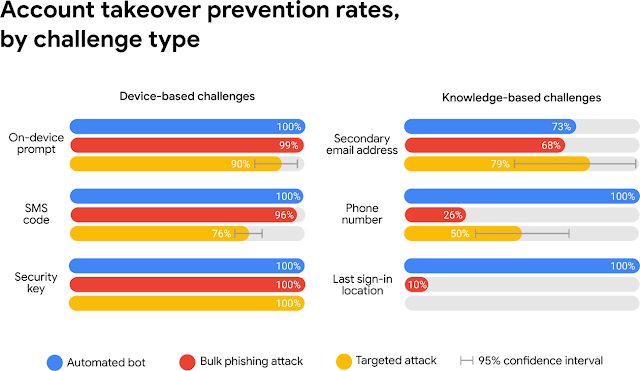
\includegraphics[width=12cm]{template/figures/account takeover provention rates.png}
    \caption{Varmentamismenetelmien tehokkuus hyökkäyksiä vastaan \citep{google_security}}
    \label{fig:account_takeover_rates}
\end{figure}

Seuraavaksi kirjautumismenetelmien soveltuvuus pankkipalveluissa. Pankkipalveluissa tärkeintä on käyttäjän henkilöllisyyden tunnistaminen ja varmentaminen. Pankkipalveluissa käsitellään raha-asioita, joka on tärkeä ja kriittinen asia. Tämän takia vain oikealla ihmisellä tulisi pelkästään olla pääsy omiin tietoihin. Tämän takia käytetään niin sanottua vahvaa tunnistautumista pankkipalveluiden kirjautumisessa. \citep{kpclient}
Suomessa pankeilla on lakisääteinen velvollisuus tunnistaa asiakkaan henkilöllisyys ennen kuin tekevät sopimuksen asiakkaan kanssa ja antaa tälle pankkitunnukset. Henkilöllisyyden todentamiseen vaaditaan virallinen henkilöllisyystodistus. Tämän pakollisen henkilöllisyyden varmentamisen avulla saadaan yhdistettyä käyttäjän pankkitunnus sekä hänen henkilöllisyytensä. Kun käyttäjä kirjautuu pankkipalveluun pankkitunnuksella, pankki pystyy yhdistämään ja varmentamaan käyttäjän henkilöllisyyden. Henkilöllisyyden varmentaminen on tärkeää koska pankkitunnusten avulla voidaan tunnistautua pankkipalveluiden lisäksi myös yksityisissä sekä viranomaisten sähköisissä palveluissa. \citep{FINE_verkkopankkitunnukset}
Pankkitunnusten vahvuus on se, että sen avulla pystytään varmentamaan käyttäjän henkilöllisyys. Täten verkkopankkitunnuksia voidaan pitää luotettava ja vahvasti suositeltavana valintana pankkipalveluissa.
Vertailun muut varmentamismenetelmät olisivat teknillisesti mahdollisia vaihtoehtoja. Mutta pankkipalveluihin kirjautuessa käyttäjän henkilöllisyyden varmentaminen on tärkeää ovat nämä menetelmät mahdollisia mutta ei suositeltavia.

Pankkipalveluiden lisäksi myös julkiset palvelut ovat tärkeitä ja kriittisiä palveluita. Julkiset palvelut on seuraava vertailtava kohde. Julkisissa palveluissa kuten Omaverossa, Omakannassa ja Opintopolussa käsitellään tärkeitä, kriittisiä ja henkilökohtaisia tietoja. Tämän takia varmentaminen näissä palveluissa on tärkeää. Palveluiden tulee olla varmistaa ja olla varma käyttäjän henkilöllisyydestä. Vain oikeilla henkilöillä on pääsy vain omiin tietoihin. Tämän takia julkisissa palveluissa käyttäjän täytyy tunnistautua luotettavasti käyttäen niin sanottua vahvaa tunnistautumista. Suomessa on käytössä suomi.fi-tunnistuspalvelu. Se on julkishallinnon asiointipalveluiden yhteinen tunnistautumispalvelu ja sen avulla voi kirjautua kaikkiin suomalaisiin julkishallinnon sähköisiin palveluihin, jotka edellyttävät vahvaa tunnistautumista. Pankkitunnukset on yksi hyväksytty varmentamismenetelmä. Pankkitunnukset on vahvasti suositeltava menetelmä. \citep{suomi.fi} 
Julkisiin palveluihin vaaditaan vahvaa tunnistautumista. Vertailun muut varmentamismenetelmät voisivat olla mahdollisia menetelmiä, mutta eivät ole suositeltavia koska käyttäjän henkilöllisyyttä ei voida vahvistaa.



IoT laitteet ovat viimeinen vertailtava käyttötarkoitus. IoT laitteet on hyvin erilainen käyttötarkoitus kuin edellä vertaillut. Edellisissä vertailuissa käyttötarkoituksena ja kohteena oli yksittäinen laite tai palvelu. Kun taas IoT laitteet koostuvat useasta joissakin tilanteissa jopa tuhansista laitteista. Tämä aiheuttaa uudenlaisen haasteen kirjautumismenetelmissä.
IoT laitteissa kuten kaikissa muissakin tutkituissa käyttötarkoituksissa turvallisuus on tärkeä asia. IoT laitteisiin kirjautuminen ja datan siirtäminen tulee tapahtua turvallisesti ja salatusti. IoT laitteissa salaus ja kirjautuminen täytyy kuitenkin olla nopeaa. Kun puhutaan tuhansista tai jopa miljoonista laitteista kirjautumiseen vaadittavan ajan merkitys kasvaa.

IoT laitteita voi olla rajaton määrä. Laitteita voi olla monenlaisia sekä erikokoisia. IoT laitteet voivat kommunikoida toistensa kanssa tai internetin kautta muihin laitteisiin. IoT laitteissa ei välttämättä ole sisäistä varmentamista ja se voi lähettää suojaamataonta dataa. IoT laitteiden kommunikointiin ei ole olemassa yhtenäisiä standardeja. IoT laitteet on siis hyvin erilainen käyttötarkoitus. IoT laitteisen salaamiseen soveltuu parhainten salaiset avaimet sekä muut yksinkertaiset menetelmät. Fyysisen avaimen käyttäminen on yksi hyvä vaihtoehto. Fyysinen avain sisältää salaisen avaimen, jolla IoT laitteisiin voidaan kirjautua ja purkaa salaus. Tämän takia fyysinen avain on vahvasti suositeltava. Myös koodiperusteiset kuten aikaan perustuva kertakäyttöinen koodi on myös mahdollinen vaihtoehto IoT laitteiden kirjautumiseen.

IoT laitteiden kirjautuminen ja salaaminen on mahdollista toteuttaa monella eri tavalla. Ei ole olemassa yhtä oikeaa vaihtoehtoa. Ensimmäiseksi voidaan todeta, että pankkitunnukset eivät sovellu tähän tarkoitukseen. Pankkitunnukset ovat epäkäytännöllinen kirjautumismenetelmä IoT laitteissa. Pankkitunnusten käyttäminen ei ole suositeltavaa käyttää muuhun kuin vahvaa tunnistautumista vaativissa palveluissa. SMS varmenne, sähköposti sekä mobiilisovellus ovat mahdollisia menetelmiä IoT laitteissa. \citep{el2019survey} \citep{lucia2019device}




Vertailuiden ja taulukkoon \ref{tab:vertailu} koostettujen arvosanojen perusteella voidaan tulkita varmentamismenetelmien soveltuvuutta. Pankkitunnukset soveltuvat parhainten käyttötarkoituksiin, joissa vaaditaan vahvaa tunnistautumista kuten pankkipalvelut ja julkiset palvelut. Pankkitunnusten hyöty on se, että käyttäjän henkilöllisyys tiedetään koska se on vahvistettu pankkitunnusten annoin aikana pankin toimesta. Pankkitunnusten käyttäminen muissa palveluissa olisi mahdollista mutta se ei ole suositeltavaa. Vahvan tunnistautumisen menetelmää tulisi käyttää vain palveluissa, joissa tämä on välttämätöntä. 

 
SMS varmenne, kertakäyttöiset koodit, fyysinen avain ja mobiilisovellus ovat suositeltavia tai jopa vahvasti suositeltavia menetelmiä monessa eri käyttötarkoituksessa.
Varmentamismenetelmistä sähköposti on pelkästään vahvasti suositeltava vaihtoehto. 
